%
% elliptic.tex -- XXX
%
% (c) 2019 Prof Dr Andreas Mueller
%
\chapter{Elliptische Differentialgleichungen\label{chapter-elliptisch}}
\index{Differentialgleichung!partielle!elliptische}
\lhead{Elliptische PDGL}
In diesem Kapitel untersuchen wir Lösungen elliptischer Differentialgleichungen
und entdecken dabei die Mittelwerteigenschaft
harmonischer Funktionen sowie die Greensche Funktion, mit der sich für
die Lösung des Randwertproblems eine Formel aufstellen lässt.
\index{Mittelwerteigenschaft}
\index{Greensche Funktion}

%
% intro.tex -- 
%
% (c) 2019 Prof Dr Andreas Mueller, Hochschule Rapperswil
%
\section{Introductory example}
\subsection{Wave equation for a vibrating string}
\rhead{Vibrating string}
We introduce the ideas to the transformation method by applying it
once more to the wave equation of the vibrating string
\[
\partial_t^2u=\partial_x^2u.
\]
The separation method gave us two ordinary differential equations
$X''=-k^2X$ and $T''=-k^2T$ with the trigonometric functions as
solutions.
Combining the linearly lead us to using the Fourier series of the
initial conditions to find the solution.

However, we could begin right away with Fourier theory and
use that any function on the interval $[0,\pi]$ can be extended
in some way to a function on $[-\pi,0]$ and further to a periodic
function on $\mathbb R$.
By using Fourier analysis at each point in time, we get a
Fourier series for the functions $x\mapsto u(t,x)$
\[
u(t,x)
=
\frac{a_0(t)}2+\sum_{k=1}^\infty \bigl( a_k(t)\cos kx+b_k(t)\sin kx \bigr)
\]
with time dependent Fourier coefficients.
Substituting this into the wave equation we get
\begin{align*}
\partial_t^2u(t,x)&=\frac{a_0''(t)}2
+\sum_{k=1}^\infty\bigl( a_k''(t)\cos kx+b_k''(t)\sin kx\bigr)\\
\partial_x^2u(t,x)&=
-\sum_{k=1}^\infty \bigl(a_k(t)k^2\cos kx+b_k(t)k^2\sin kx \bigr)
\end{align*}
If these functions are the same the equations
the equation
\[
\frac{a_0''(t)}2
+\sum_{k=1}^\infty (a_k''(t)+k^2a_k(t))\cos kx+(b_k''(t)+k^2b_k(t))\sin kx=0
\]
must hold.
According to Fourier theory, this is only possible of all the coefficients
are $0$:
\begin{align*}
a_0''(t)&=0\\
a_k''(t)&=-k^2a_k(t)\\
b_k''(t)&=-k^2b_k(t)
\end{align*}
with $k>0$.
Thus by going to Fourier coefficients, a system of ordinary differential
equations for the Fourier coefficents was found.
The solution of these ordinary differential equations are well known:
\begin{align*}
a_0(t)&=m_0t+c_0\\
a_k(t)&=A^a_k\cos kt+B^a_k\sin kt\\
b_k(t)&=A^b_k\cos kt+B^b_k\sin kt
\end{align*}
These are the solutions that we have found in the previous chapter.
The parameters $A$ and $B$ need to be found from initial conditions.

\subsection{Initial conditions}
The differential equations for the coefficients $a_k(t)$ and $b_k(t)$
require some initial conditions in order for us to solve them uniquely.
Let's assume that the initial conditions are given in the form
\begin{align*}
u(0,x)&=f(x)\\
\frac{\partial u}{\partial t}&=g(x).
\end{align*}
The functions $f$ and $g$ can also be represented as Fourier series,
we write them as
\begin{align*}
f(x)&=\frac{a_0^f}2+\sum_{k=1}^\infty \bigl( a_k^f\cos kx+b_k^f\sin kx \bigr)\\
g(x)&=\frac{a_0^g}2+\sum_{k=1}^\infty \bigl( a_k^g\cos kx+b_k^g\sin kx \bigr).
\end{align*}
Together with the solution $u(t,x)$ written as a Fourier series 
we can now identify the coefficients by substiting $u(0,x)$ in
the initial conditions
\begin{align*}
\frac{a_0(0)}2+\sum_{k=1}^\infty \bigl( a_k(0)\cos kx +b_k(0)\sin kx \bigr)
&=
\frac{a_0^f}2+\sum_{k=1}^\infty \bigl( a_k^f\cos kx+b_k^f\sin kx \bigr)\\
\\
\frac{a_0'(0)}2+\sum_{k=1}^\infty \bigl( a_k'(0)\cos kx+b_k'(0)\sin kx \bigr)
&=
\frac{a_0^g}2+\sum_{k=1}^\infty \bigl( a_k^g\cos kx+b_k^g\sin kx \bigr).
\end{align*}
Comparing coefficients not gives us the initial conditions
for the functions $a_k(t)$ and $b_k(t)$:
\begin{align*}
a_k(0)&=a_k^f&b_k(0)&=b_k^f\\
a_k'(0)&=a_k^g&b_k'(0)&=b_k^g
\end{align*}
Using the previously found solutions we get
\begin{align*}
c_0&=a_0^f&&&A_k^a&=a_k^f&&&&&A_k^b&=b_k^f\\
m_0&=a_0^g&&&kB_k^a&=a_k^g&\Rightarrow B_k^a&=\frac1ka_k^g&&&kB_k^b&=b_k^g&\Rightarrow B_k^b&=\frac1kb_k^g.
\end{align*}
The complete solution thus is
\begin{align*}
u(t,x)=\frac{a_0^gt+a_0^f}2
+\sum_{k=1}^\infty \biggl(
\bigl(a_k^f\cos kt+{\textstyle\frac1k}a_k^g\sin kt\bigr)\cos kx
+
\bigl(b_k^f\cos kt+{\textstyle\frac1k}b_k^g\sin kt\bigr)\sin kx
\biggr).
\end{align*}

\subsection{Inhomogeneous wave equation}
The method can be generalized to the inhomogeneous wave equation
\[
\partial_t^2u-\partial_x^2u=f.
\]
The partial function $x\mapsto f(t,x)$ can also be written 
as a Fourier series in the variable $x$ just as we did for $u$:
\[
f(t,x)
=
\frac{a_0^f(t)}2
+
\sum_{k=1}^\infty \bigl( a_k^f(t)\cos kx+b_k^f(t)\sin kx \bigr).
\]
Substituting this into the inhomegeneous wave equation gives
\begin{align*}
a''_k(t)+k^2a_k(t)&=a_k^f(t)\\
b''_k(t)+k^2b_k(t)&=b_k^f(t),
\end{align*}
again a system of ordinary differential equations.
While the previous set of ordinary differential equations was linear
and homogeneous, the new set of equations is inhomogeneous.

\subsection{Lessons learned from the introductory example}
The transform to Fourier coefficients makes derivatives with respect
to $x$ disappear, instead what remains is a family of ordinary
differential equations.
The second derivative with respect to $x$ becomes the algebraic
operation of multipication by $-k^2$.
This transform was possible because the $x$-domain was an interval.
For other $x$-domains, this method will not work.


%
% unique.tex -- 
%
% (c) 2019 Prof Dr Andreas Mueller
%
\section{Uniqueness of a solution}
We now study the question whether the solution of the Dirichlet problem
\eqref{elliptisch:laplaceequation} and \eqref{dirichletrandbedingung},
if they exist, is unique.

Let $u_1$ and $u_2$ be two solutions of the problem.
The difference satisfies
\[
\begin{aligned}
\Delta u&=\Delta u_1-\Delta u_2=f-f=0&&\text{in $\Omega$,}\\
u&=u_1-u_2=g-g=0&&\text{on $\partial\Omega$.}
\end{aligned}
\]
$u$ is a solution of the homogeneous problem with homogeneous 
boundary conditions.

This observation holds true for any other linear partial differential
operator of the form
\[
L=\sum_{i,j}a_{ij}\partial_i\partial_j+\sum_i b_i\partial_i.
\]
Uniqueness of solutions is thus equivalent to uniqueness of solutions
of the homogeneous problem with homogeneous boundary conditions.
This follows from the following theorem:
eindeutige Lösung hat. Dies wiederum folgt aus dem folgenden Satz.

\begin{satz}[Maximum principle for elliptic operators]
\label{maximumprinzip}
If $L$ is an elliptic differential operator on a connected and
bounded domain $\Omega$, and $u$ is a solution $Lu=0$, then $u$ takes
its maximum and minimum on the boundary of $\Omega$.
\end{satz}

The condition that the domain $\Omega$ needs to be bounded is essential.
The function $u(x,y)=x$ is harmonic, $\Delta x=0$, on the domain
$\Omega=\{(x,y)\,|\,x>0\}$, and it vanishes on the boundary, which is
the $y$-axis, where we have $u(0,y)=0$.
So this $u$ is a solution of the Poisson problem with homogeneous
Dirichlet boundary conditions with homogeneous boundary conditions, 
but it does not take a maximum anywhere.

The connectedness of the domain es essential too.
Define the function
\[
u(x)=n\qquad\text{für $2^{-n} < |x| < \frac{3}{2}2^{-n}$},
\]
then $\Delta u=0$, it is constant on rings around the origin and hence
$u$ is harmonic.
The values of $u$ are not bounded as there are infinitely many disjoint
rings.
In particular, there is no maximum.

\begin{proof}[Proof idea]
We prove the theorem with the help of a constradiction.
We assume that $u$ takes a maximum in some interior point $x$
in $\Omega$.

We may assume that the matrix $a_{ij}$ is diagonal that, as $L$
is elliptic, that $a_{ii}=\lambda_i$ are all positive.
As $u$ has a maximum in $x$, all first order derivatives vanish
in $x$ and at least one of the second derivatives
must be nagative:
\[
\frac{\partial^2u}{\partial x_i^2}
\le 0
\quad
\Rightarrow
\quad
\sum_{i}\lambda_i \frac{\partial^2u}{\partial x_i^2} \le 0
\quad
\Rightarrow
\quad
Lu<0
\]
This contradiction shows that there cannot be a maximum in the
interior of the domain.

However, this is unfortunately not a proof.
There is no reason why not all second derivatives of $\partial^2_{x_i} u$ 
could be zero.
We give a complete proof at the end of this section.
\end{proof}

\begin{satz}
There is at most one solution of
$Lu=f$ 
with boundary conditions
$u_{|\partial\Omega}=g$.
\end{satz}

\begin{proof}
Let $u_1$ und $u_2$ be solutions, then $u=u_1-u_2$ is a solution of
$Lu=0$ with boundary conditions $u_{|\partial\Omega}=0$.
According to theorem \ref{maximumprinzip} $u$ takes its maximum and
minimum on the boundary, so $0\le u\le 0$ in $\Omega$.
Consequently $u=0$ or $u_1=u-2$, it is therefore impossible that
there are two different solutions.
\end{proof}

{\small
\subsubsection{A proof of the maximum principle}
In the following we give a complete proof promised for the maximum principle.
The essential point of the proof idea was that $Lu=0$ but in an internal
maximum we could conclude $Lu<0$.
But the method we employed was only real capable of concluding that
$Lu\le 0$.
Our argument so far only proofs the following statement:
\begin{satz}
\label{maximumgt}
If $L$ is an elliptic differential operator on a connected and
bounded domain $\Omega$ and $u$ a function with the property $Lu>0$, then
$u$ takes a maximum on the boundary.
\end{satz}

This allows us to conclude:
\begin{satz}
If $L$ is an elliptic differential operator on a conneted and
bounded domain $\Omega$ and $u$ is a function with $Lu\ge > 0$,
then $u$ takes its maximum on the boundary.
\end{satz}

\begin{proof}
As in the proof sketch, we may assume that in the point $x$ the 
coefficient matrix $(a_{ij})$ is diagonal with all diagonal elements
positive.
Let $u_{\varepsilon}$ be the function
$u_{\varepsilon}=u-\varepsilon e^{\lambda x_1}$.
We get
\begin{align*}
Lu_{\varepsilon}&=Lu-\varepsilon L(e^{\lambda x_1})\\
&=Lu-\varepsilon(a_{11}\lambda^2+b_1\lambda)e^{\lambda x_1}
\end{align*}
Because $a_{11}>0$,
the quadratic polynomial $a_{11}\lambda^2+b_1\lambda$ will be positive
for sufficnently large $\lambda$.
Thus
\[
Lu_{\varepsilon}= Lu-\varepsilon(a_{11}\lambda^2+b_1\lambda)e^{\lambda x_1}<0
\]
for every $\varepsilon$.
According to theorem \ref{maximumgt},
the maximum of $u_\varepsilon$ is reached on the boundary.

In the limit $\varepsilon\to 0$ we have $u^\varepsilon\to u$, so
$u$ too must reach a maximum on the boundary.
\end{proof}

Applying this theorem to the function $-u$, the minimum principle follows:
\begin{satz}
If $L$ is an elliptic differential operator on a connected and
bounded domain $\Omega$ and $u$ a function with $Lu\le 0$, then
$u$ takes a minimum on the boundary.
\end{satz}

For solutions of $Lu=0$ the theorem \ref{maximumprinzip} follows.
}


%
% inverse.tex -- 
%
% (c) 2019 Prof Dr Andreas Mueller
%
\section{Does there exist an operator inverse to $\Delta$?}
\rhead{Does there exist $\Delta^{-1}$?}
We want to solve the problem $\Delta u=f$.
If we had an inverse operator $\Delta^{-1}$, we could use it to
find the solution $u=\Delta^{-1}f$.
This dream is too good to be true, but the examples below 
illustrate that for elliptic operators there is at least a partial
realization of it.

\subsection{Derivative and Integration}
The equation 
\[
u''(x)=f(x)
\]
in one dimension can be solved by simple integration.
To this effect we need to find an antiderivative $F$ of $f$, i.~e.~$F'=f$
and then an antiderivative $u$ of $F$.
In spite of $u''(x)=F'(x)=f(x)$, $u$ need no be a solution because
it does not satisfy the boundary conditions.

\subsection{Linear equations}
By discretization the differential equation $u''=f$ on the interval
$[a,b]$ can be turned into a linear system of equations of
the form $Au=f$.
The components of $u$ and $f$ are values of the functions of $u$ and $f$
in selected points of the domain.
And since we have seen that the solution is unique for elliptic operators,
there should be an inverse matrix $G$ that can be used to find the
solution in the form $u=Gf$.

The matrix product is
\[
\sum_{j}g_{ij}f_j = u_i,
\]
and the $g_{ij}$ can also be considred to be values of a function $G(x,y)$
defined in particular points of $\Omega\times\Omega$.

If the points used for discretization come closer together, the sum
can ultimately better be approximated by an integral of the form
\[
u(x)=\int_a^b G(x,\xi)f(\xi)\,d\xi.
\]
So we are left with the question whether there actually exists such
a function $G(x,\xi)$.
Still, there is no guarantee that this will be a solution, as
the boundary conditions may not be satisfied.

\subsection{Boundary conditions}
The boundary conditions also enter linearly into the problem.
In the one dimensional problem we have two points on the boundary
so we expect a contribution of the form
\[
K(x,a) g(a) + K(x,b)g(b),
\]
where $K(x,\xi)$ is another function defined on $x\in [a,b]$ and
$\xi \in\{a,b\}=\partial[a,b]$.
If the boundary is more complicated and consists of multiple points,
the contribution generalizes to a sum
\[
\sum_{i}K(x,a_i)g(a_i),
\]
where all the points $a_i$ are on the boundary.
Again, with the boundary becoming a curve or surface, the
contribution of the boundary values must be computed with
the help of an integral
\[
\int_{\partial\Omega}K(x,\xi)g(\xi)\,d\xi
\]
over the boundary of the domain.
So we expect a solution in the form
\begin{equation}
u(x)=\int_{\Omega} G(x,\xi)f(\xi)\,d\xi + \int_{\partial\Omega} K(x,\xi)g(\xi)\,d\xi.
\label{greenformula}
\end{equation}
The goal of the subsequent sections is to show that in some cases,
such functions actually exists.


%
% 1dim.tex -- 
%
% (c) 2019 Prof Dr Andreas Mueller
%
\section{The one-dimensional problem}
\rhead{The one-dimensional case}
As a demonstration that the program sketched in the previous section
may actually be implemented, we consider the one dimensional problem
\[
u''(x)=f(x)
\]
on the interval $[0,1]$ with boundary conditions
\[
u(0)=a,\quad u(1)=b.
\]
The goal is to find the function $G(x,\xi)$.

THe solution of this problem usually is treated in the theory of
ordinary differential equations.
Here we would slightly modify the presentation in such a way
that it leads to $G$ and is more easily generalizable to 
multiple independent variables.

\subsection{Particular solution}
It is easy to find a particular solution, just take an antiderivative
of $f$ as in
\begin{align*}
u_p'(x)&=\int_0^xf(\xi)\,d\xi,
\\
u_p(x)&=\int_0^xu_p'(\eta)\,d\eta=\int_0^x\int_0^\eta f(\xi)\,d\xi\,d\eta.
\end{align*}
However, this solution does not satisfy the boundary conditions.
For this we have to add a suitable solution of the homogeneous
equation
\[
u_p''(x) + u_r''(x)=f(x)\quad\Rightarrow\quad u_r''(x)=0
\]
with boundary conditions
\begin{align*}
u_r(0)&=a-u_p(0)=a\\
u_r(1)&=b-u_p(1)=b-\int_0^1\int_0^\eta f(\xi)\,d\xi\,d\eta
\end{align*}

\subsection{The homogeneous problem}
The homogeneous problem
\[
u''(x)=0
\]
is even easier to solve.
The general solution is $Ax+B$, and the constants have to chosen
so that the boundary conditions hold, i.~e.
\begin{align*}
A\cdot 0+B&=a\qquad\Rightarrow&B&=a\\
A\cdot 1+B&=b\qquad\Rightarrow&A&=b-a
\end{align*}
which leads to $u(x)=(b-a)x+a=(1-x)a+xb$.

\subsection{General solution}
In the present example, $u_r$ is expected to take the boundary value
$b-\int_0^1\int_0^\eta f(\xi)\,d\xi\,d\eta$
für $x=1$, i.~e.
\[
u_r(x)=(1-x)a+x\left(b-\int_0^1\int_0^\eta f(\xi)\,d\xi\,d\eta\right).
\]
The complete solution thus becomes
\begin{align}
u(x)&=u_p(x)+u_r(x)\notag
\\
&=\int_0^x\int_0^\eta f(\xi)\,d\xi\,d\eta+(1-x)a+x\left(b-\int_0^1\int_0^\eta f(\xi)\,d\xi\,d\eta\right)\notag
\\
&=
(1-x)a+xb
+\int_0^x\int_0^\eta f(\xi)\,d\xi\,d\eta
-x\int_0^1\int_0^\eta f(\xi)\,d\xi\,d\eta\notag
\\
&=
(1-x)a+xb
+\int_0^1\vartheta(x-\eta)\int_0^1 \vartheta(\eta - \xi)f(\xi)\,d\xi\,d\eta
-x\int_0^1\int_0^1\vartheta(\eta-\xi) f(\xi)\,d\xi\,d\eta\notag
\\
&=
(1-x)a+xb
+\int_0^1\int_0^1
(\vartheta(x-\eta)-x)\vartheta(\eta -\xi)
f(\xi)\,d\xi\,d\eta
\notag
\\
&=
(1-x)a+xb+\int_0^1\int_0^1
(\vartheta(x-\eta)-x)\vartheta(\eta -\xi)
\,d\eta\,
f(\xi)\,d\xi
\label{1dimgreen}
\end{align}
By $\vartheta(t)$ we mean the step function
\[
\vartheta(t)=\begin{cases}
0&\qquad t<0\\
1&\qquad t\ge 0,
\end{cases}
\]
also called the Heaviside function.
The function $\vartheta(x-\xi)$ vanishes as soon as $\xi$ surpasses
$x$ because in that case $x-\xi<0$.

We now have to convert the expression \eqref{1dimgreen} into a form
that exhibits Green's function $G$.
The inner integral of \eqref{1dimgreen} can easily be done:
\begin{align*}
\int_0^1(\vartheta(x-\eta)-x)\vartheta(\eta-\xi)\,d\eta
&=
\int_\xi^1\vartheta(x-\eta)-x\,d\eta
\\
&=
\int_\xi^1\vartheta(x-\eta)\,d\eta-\int_\xi^1x\,d\eta
\\
&=
\int_\xi^1\vartheta(x-\eta)\,d\eta-(1-\xi)x
\end{align*}
The second integral requires a distinction of two possible cases:
\begin{align*}
\int_\xi^1\vartheta(x-\eta)\,d\eta
&=
\begin{cases}
\int_\xi^x\,d\eta=x-\xi&\qquad\eta>\xi\\
0&\qquad x\le \xi
\end{cases}
\\
&=(x-\xi)\vartheta(x-\xi)
\end{align*}
All together we find the following function for the inner integral.
\[
G(x,\xi)=(x-\xi)\vartheta(x-\xi)-x(1-\xi).
\]
It is also possible to write this function using the 
absolute value function
The partial function $x\mapsto h(x,\xi)$ is not differentiable at $\xi$
but on both sides it is the linear function
\[
G(x,\xi)=\begin{cases}
(x-\xi)-x(1-\xi)=\xi(x-1)&\qquad x>\xi\\
x(\xi-1)&\qquad x<\xi
\end{cases}
\]
we want to write this in the form $c|x-\xi|+dx+e$, which requires
some computation for the coefficients $c$, $d$ and $e$.
The result turns out to be
\[
G(x,\xi)
=
{\textstyle \frac12}|x-\xi|-({\textstyle \frac12}-\xi)x-{\textstyle\frac12}\xi.
\]
The second and third terms on the right hand side is a linear function
of $x$ which does not contribute anything to the second derivative.
So outside the point $x=\xi$, the second derivative of $G$ with respect 
to $x$ vanishes.

The derivative of the first term is a step function with step
height $1$:
\[
\frac{\partial}{\partial x}({\textstyle \frac12}|x-\xi|)
=
\vartheta(x-\xi)
-
{\textstyle\frac12},
\]
and the derivative of this is the $\delta$ function
\[
\frac{\partial^2}{\partial x^2}({\textstyle \frac12}|x-\xi|)
=
\delta(x-\xi).
\]
Thus the essential part is the function
\begin{equation}
\sigma(x,\xi)=\frac12|x-\xi|.
\label{n1sigma}
\end{equation}

\subsection{Green's function}
\begin{figure}
\begin{center}
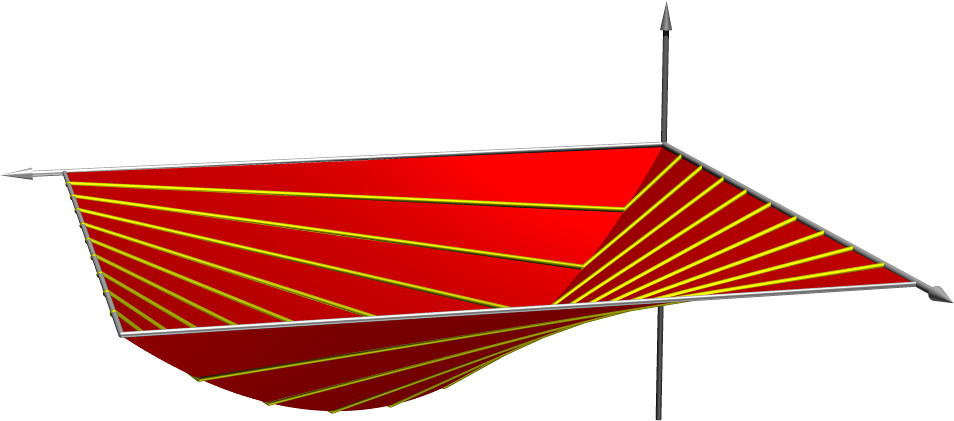
\includegraphics[width=\hsize]{../common/3d/green.jpg}
\end{center}
\caption{Graph of Green's function $G(x,\xi)$ for the problem $u''=f$ 
on the interval $[0,1]$ as a surface over the square $(x,\xi)\in[0,1]^2$.
For each value $\xi$ the partial function
$x\mapsto G(x,\xi)$ is a solution of the differential equation
$u''=\delta_\xi$ with boundary condition $u(0)=u(1)=0$.
\label{elliptisch:green3dflaeche}}
\end{figure}
\begin{figure}
\begin{center}
\includegraphics{../common/images/green-1.pdf}
\end{center}
\caption{Partial function $x\mapsto G(x,\xi)$ of Green's function
for the problem $u''=f$ with boundary conditions 
$u(0)=u(1)=0$ for various values of $\xi$.
\label{elliptisch:green1schar}}
\end{figure}

The formular for the solution $u(x)$ we have found writes the solution
as a double integral, but this is not the form we are looking for.
We want the solution as a simple integral over $[0,1]$ with integrand
$G(x,\xi) f(\xi)$.

We can use the function $h$ to fix this.
The partial function $x\mapsto h(x,\xi)=(x-\xi)\vartheta(x-\xi)$ has boundary
values $0$ and $1-\xi$, so the function
\[
G(x,\xi)
=
(x-\xi)\vartheta(x-\xi)-x(1-\xi)
=\begin{cases}
(x-\xi)+x(\xi-1)&\qquad x\le \xi \\
x(\xi-1)&\qquad x<\xi
\end{cases}
\]
has both boundary values equal to $0$.
$G$ satisfies
\[
\frac{\partial^2}{\partial x^2}G(x,\xi)=\delta(x-\xi)
\]
and
\[
G(0,\xi)=G(1,\xi)=0.
\]
A solution of the differential equation can thus be written as
\[
u(x)=\int_0^1G(x,\xi)f(\xi)\,d\xi+a(1-x)+bx.
\]

The ondimensional case shows that for the operator  $D^2$ and the
equation $D^2u=f$
we can actually find a function $G(x,\xi)$ that takes the role 
of an inverse.

Figures~\ref{elliptisch:green3dflaeche} and \ref{elliptisch:green1schar}
show Green's function $G(x,\xi)$.
The partial functions 
$x\mapsto G(x,\xi)$ are solutions of the problem
$u''=\delta_\xi$ with boundary conditions $u(0)=u(1)=0$.
In both figures, the partial functions are highlighted for 
a number of special values $\xi$.

\begin{beispiel}
The differential equation
\[
y''=\cos 3\pi x.
\]
has the solution
\[
y(x)=-\frac1{9\pi^2}(\cos 3\pi x + 2x - 1),
\]
which we can also find using Green's function:
\[
y(x)=\int_0^1 G(x,\xi)\cos 3\pi\xi\,d\xi.
\]
In figure~\ref{elliptisch:green-beispiele}
the right hand side $f(x)=\cos 3\pi x$ is approximated as a linear
combination of $\delta$-distributions (blue).
The associated solution is shown in red, it has kinks at each 
contributing $\delta$-function.
Increasing the number of $\delta$ functions produces better approximations
of the solution.
\begin{figure}
\begin{center}
\includegraphics[width=0.7\hsize]{../common/graphics/green-1.pdf}\\
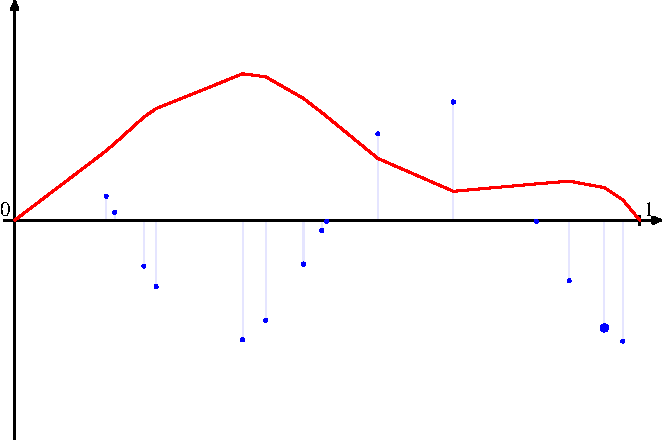
\includegraphics[width=0.7\hsize]{../common/graphics/green-324.pdf}\\
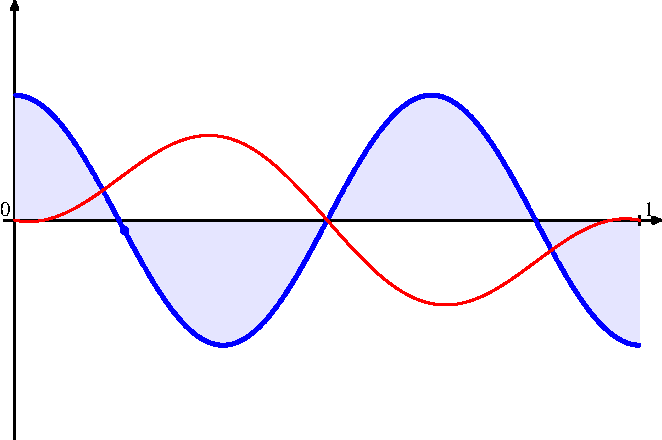
\includegraphics[width=0.7\hsize]{../common/graphics/green-1082.pdf}
\end{center}
\caption{Solution (red) of $y''=f$ and for an approximation of $f$ by
$\delta$-distributions (blue).
\label{elliptisch:green-beispiele}}
\end{figure}

An animation for the computation of $y(x)$ using Green's function
can be found on Youtube:
\url{http://www.youtube.com/watch?v=Wpi7Gf7V2HY}
\end{beispiel}


%
% general.tex -- 
%
% (c) 2019 Prof Dr Andreas Mueller
%
\section{The general case}
\rhead{The general case}
We now want to solve the general case of the problem
\[
\begin{aligned}
\Delta u&=f&&\text{in $\Omega$}\\
u&=g&&\text{auf $\partial\Omega$}
\end{aligned}
\]
using an integral formula of the kind
\eqref{greenformula}.
Following the one dimensional case, we are looking for a particular
solution $G(x,\xi)$ for the problem with a $\delta$-distribution on
the right hand side.
Once such a solution is found, we can find solutions for the general
problem using an integral formular.

\subsection{A particular solution}
\rhead{Particular solution}
The one-dimensional sample problem suggests that there is a function
$\sigma(x,\xi)$, which allows to find a particular solution of the
Laplace equation using the integral
\begin{equation}
u_p(x)=\int_\Omega \sigma(x,\xi)  f(\xi)\,d\xi.
\label{singulaereloesunglaplace}
\end{equation}
This particular solution does not need to satisfy the boundary conditions,
we just require that $\Delta u=f$ holds.

The solution $\sigma$ does not have to depend on the shape of the domain,
as it does not have to respect any boundary conditions,
but it will change with the dimension $n$.
If we choose the right hand side $f$ to be a $\delta$ distribution in the
point $y$, then
\[
u(x)
=
\int_\Omega \sigma(x,\xi)\delta(\xi - y)\,d\xi
=
\sigma(x,y).
\]
Thus the partial function $x\mapsto \sigma(x,y)$ satisfies the equation
$\Delta \sigma(x,y)=0$ for all points in ${\mathbb R}^n\setminus\{y\}$.
The function $\sigma$ thus is a harmonic function in the set
$\mathbb R^n\setminus\{y\}$.

Determining the function $\sigma(x,y)$ is a bit tedious, we just give the
result.
We find\footnote{%
This solution can be found using the following argument.
First the solution should only depend on the distance $|x-\xi|$, which
means we can assume without losing any generality that $\xi=0$.
As $\Delta u=\operatorname{div}\operatorname{grad}u$ we  conclude using
Gauss' theorem that
\begin{align*}
1&=\int_{B_r^n} \Delta u(x)\,d\mu(x)
=
\int_{B_r^n} \operatorname{div}\operatorname{grad} u(x)\,d\mu(x)
=\int_{S_r^{n-1}}\operatorname{grad}u(x)\cdot dn
\\
&=\int_{S_r^{n-1}}|\operatorname{grad}u(x)|\,d\mu(x)
=\mu(S_r^{n-1})\left|\frac{d}{dr}u(r)\right|
\\
\Rightarrow\qquad\frac{d}{dr}u(r)
&=\frac1{\mu(S_r^{n-1})}
=\frac1{\mu(S_1^{n-1})r^{n-1}}.
\end{align*}
For $n=2$ we have
$\mu(S_r^1)=2\pi r$, which implies
\[
u'(r)=\frac1{2\pi r}\quad\Rightarrow\quad u(r)=\frac1{2\pi}\log|r|.
\]
For $n\ge 3$ we get
\[
u'(r)=\frac1{\mu(S^{n-1})}r^{1-n}\quad\Rightarrow\quad u(r)=\frac1{\mu(S^{n-1})}\cdot \frac1{2-n}r^{2-n}.
\]
}
\begin{equation}
\sigma(x,\xi)=
\begin{cases}
\displaystyle \frac12|x-\xi|
&\qquad \text{for $n=1$}
\\
\\
\displaystyle \frac1{2\pi}\log|x-\xi|
&\qquad \text{for $n=2$}
\\
\\
\displaystyle -\frac1{4\pi}\frac1{|x-\xi|}
&\qquad \text{for $n= 3$}
\\
\\
\displaystyle \frac1{(2-n)\mu(S^{n-1})}|x-\xi|^{2-n}
&\qquad \text{for $n\ge 3$}
\end{cases}
\end{equation}
For $n=1$ we already have determined this function in \eqref{n1sigma}.
By carefully performing all these derivatives we can verify
that these functions are in fact solutions and that
\eqref{singulaereloesunglaplace} is particular solution of
Laplace equation.

\subsection{Green's function}
The propsed $\sigma$ is of course not the only function for which
the formula \eqref{singulaereloesunglaplace} will give a particular solution.
By adding any function $h(x,\xi)$ which is harmonic as a function of $x$
the integral
\[
u(x)=\int_{\Omega}\sigma(x,\xi)f(\xi)\,d\xi-\int_{\Omega}h(x,\xi)f(\xi)\,d\xi
\]
will also be a solution of
\eqref{elliptisch:laplaceequation}.
In particular we can choose $h(x,\xi)$ in such a way that
the partial function
$x\mapsto h(x,\xi)$
solves the boundary value problem
\[
\begin{aligned}
\Delta_x h(x,\xi)&=0&&x\in\Omega\\
h(x,\xi)&=\sigma(x,\xi)&&x\in\partial\Omega.
\end{aligned}
\]
The function $h$ then has the same boundary values as $\sigma$.
Consequently the difference $\sigma(x,\xi)-h(x,\xi)$ is a function
that vanishes on the boundary $\partial\Omega$.
The solution $u(x)$ found using \eqref{singulaereloesunglaplace}
then also vanishes on the boundary.
We set
\[
G(x,\xi)=\sigma(x,\xi)-h(x,\xi)
\]
and call this the Green's function for the Poisson problem on the
domain $\Omega$.

\begin{satz}If $\Omega$ is a domain on which the Poisson problem
has unique solutions, then there is a function $G(x,\xi)$,
which, as a function $x$, solves the equation
\[
\Delta G(x,\xi)=\delta(x-\xi)
\]
with homogenous boundary conditions.
\end{satz}

Note that this theorem guarantees the existence of Green's function 
but does not provide a method to obtain it.
Green's function deends only on the shape of the domain, not on
the actual boundary condtions.
Since there are domains where the Poisson problem with Dirichlet
boundary conditions cannot be solved in a unique way, the theorem
needs to require this as a precondition.

Green's function for the Poisson problem solves the problem
not only for homogeneous ($g=0$) boundary conditions, sondern
for any boundary values $g\ne 0$:

\begin{satz}[Solution of Poisson problem with Dirichlet boundary conditions]
\label{dirichletloesung}
If $G$ is Green's function for the Poisson problem with Dirichlet
boundary values on the domain $\Omega$, then
\[
u(x)
=
\int_{\Omega}G(x,\xi)f(\xi)\,d\mu(\xi)
+
\int_{\partial\Omega}g(\xi)\operatorname{grad}_\xi G(x,\xi)\cdot dn
\]
is the solution for the same problem with arbitrary boundary values
\eqref{dirichletrandbedingung}.
\end{satz}

Note that is very much in line with what we have found for the one
dimensional case.
The terms of \eqref{elliptic:greendiff} containing the derivatives
of $G$ can be considered as the integral of the gradient of $G$
over the bounary of the interval, which would be computed as a sum
of the values in the boundary points.

\begin{proof}
We already know that the integral over $\Omega$ is a solution of the
inhomogeneous partial differential equation with homogeneous boundary
conditions.
What remains is to show that the second term is a harmonic function,
i.~e.~it solves the homogeneous differential equation,
with boundary values $g$.

For this proof we need the following identity
\begin{align*}
\operatorname{div}(u\operatorname{grad}v)
&=
\sum_i\partial_i(u\partial_iv)
\\
&=\sum_i(\partial_iu)(\partial_iv)+\sum_iu\partial_i^2v
\\
&=\operatorname{grad}u\cdot\operatorname{grad}v+u\Delta v,
\end{align*}
from which we can derive
\[
u\Delta v-v\Delta u
=
\operatorname{div}(u\operatorname{grad}v-v\operatorname{grad}u).
\]

We apply these identities to the function $u(\xi)$ and 
to Green's function $\xi\mapsto v(\xi)=G(x,\xi)$:
\[
u(\xi)\Delta G(x,\xi)-G(x,\xi)\Delta u
=
\operatorname{div}(u\operatorname{grad}G(x,\xi)-G(x,\xi)\operatorname{grad}u)
\]
Integrating both sides over $\Omega$ and applying Gauss' theorem to
the right hand side gives
\begin{align*}
\int_{\Omega}u(\xi)\delta(\xi - x)-G(x,\xi)f(\xi)\,d\mu(\xi)
&=
\int_{\Omega}\operatorname{div}(u(\xi)\operatorname{grad}G(x,\xi)-G(x,\xi)\operatorname{grad}u)\,d\mu(\xi)
\\
u(x)-\int_{\Omega}G(x,\xi)f(\xi)\,d\mu(\xi)
&=\int_{\partial \Omega}u(\xi)\operatorname{grad}G(x,\xi)-G(x,\xi)\operatorname{grad}u(\xi)\cdot dn
\end{align*}
The second term on the right vanishes becuase $G(x,\xi)$ was chosen so
that the boundary values vanish.
In the left term we can replace $u(\xi)$ by the boundary values $g(\xi)$.
What remains is
\[
u(x)
=
\int_{\Omega}G(x,\xi)f(\xi)\,d\mu(\xi)
+
\int_{\partial\Omega}g(\xi)\operatorname{grad}G(x,\xi)\cdot dn,
\]
as claimed.
\end{proof}

\subsection{Application}
\rhead{Application}
\begin{figure}
\begin{center}
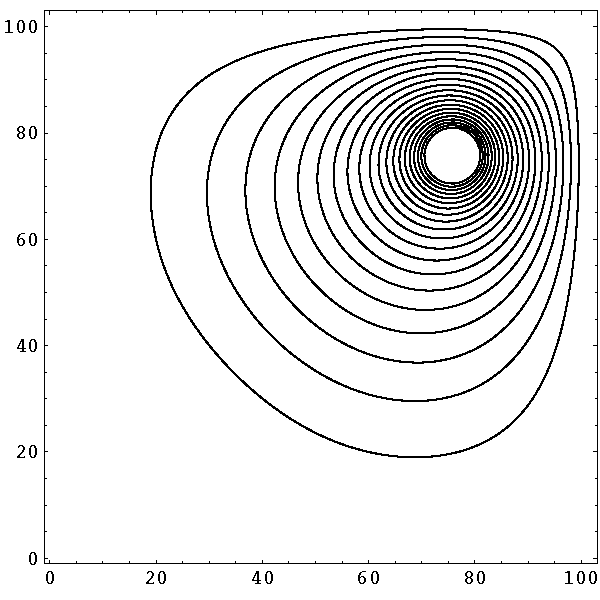
\includegraphics[width=0.8\hsize]{../common/graphics/neilcontour}
\end{center}
\caption{Level lines\label{neilcontour}}
\end{figure}
\begin{figure}
\begin{center}
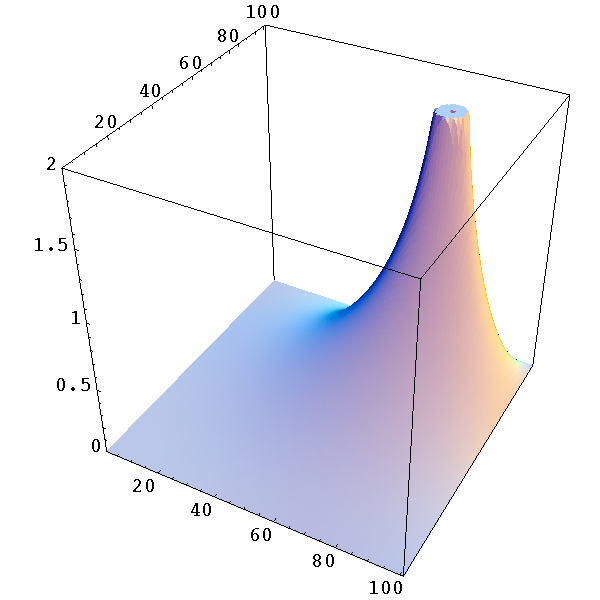
\includegraphics[width=0.8\hsize]{../common/graphics/neilloesung}
\end{center}
\caption{Potential surface\label{neilloesung}}
\end{figure}
This example illustrates how the ideas in this section can be used
to solve some practical problems at least using some numerical tool.

{\parindent 0pt
\medskip
{\bf Problem:}
The boundary of an electricaly conducting rectangular plate is connected
to the negative terminal of a battery and at the point
$x_0\in\mathbb R^2$ in the interior of the plate, the other terminal
of the battery is connected.
Compute the potential at any point $x$ of the plate with respect to
the boundary.

\medskip
}
The potential
$u(x,y)$
we are looking for is the solution of the equation
\[
\Delta u=\delta(x-x_0)
\]
with boundary values
\[
u(x)=0.
\]
Numerical computation of the solution in the vicinity of the point $x_0$
is very imprecise.
This motivates the following procedure.
The function $\sigma(x,x_0)$ is a harmonic function outside $x_0$,
\[
\Delta\sigma(x,x_0)=\delta(x-x_0)
\]
So appart from the boundary values that are not correct it could be
a solution.
So the next step is to fix the boundary values of this partial solution.
For this we solve the boundary value problem
\begin{align*}
\Delta h(x)&=0&&x\in\Omega\\
h(x)&=\sigma(x,x_0)&&x\in\partial\Omega,
\end{align*}
which can be done efficiently with existing software.
E.~g.~we could use the mean value property to be discussed later in this
chater to numerically compute such a solution.
Then the function
\[
u(x)=\sigma(x,x_0)-h(x)
\]
is a solution of the original problem.
The level lines of this solutions and the potential surface of $u(x)$ is
shown in figures~\ref{neilloesung} and \ref{neilcontour}.


%
% mean.tex -- 
%
% (c) 2019 Prof Dr Andreas Mueller
%
\section{The mean value property of harmonic functions}
\rhead{Mean value property}
Harmonic functions have a property that is even stronger than
the maximum principle for elliptic operators.
The maximum principle says that the solution of a homogeneous elliptic
partial differential equation is bounded above and below by the
extreme values on the boundary.
The mean value property in addition says that the value in some
point is actually the mean of all the values in small circle
around the point.

\subsection{Mean value property}
In this section we are going to illustrate that the values of harmonic
functions are means of the values of the function on a sphere around 
the point.
\begin{figure}
\centering
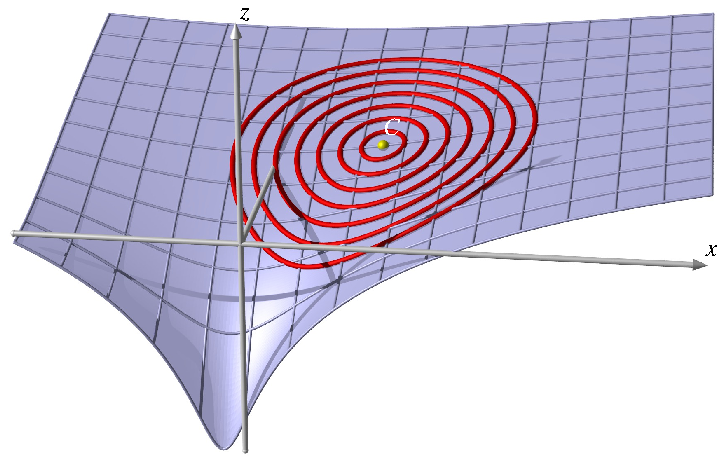
\includegraphics{7-elliptic/images/meanvalue.pdf}
\caption{Mean value property of a harmonic function.
The surface represents a harmonic function. 
The mean value along each of the red circles gives the same value,
namely the function value in the yellow center point $C$.
\label{elliptic:meanvalue:image}}
\end{figure}

\begin{satz}[Mean value property]
Let $u$ be a harmonic function on $\Omega$ and $x_0\in\Omega$.
If $r$ is small enough so that the sphere with radius $r$ in $x_0$
fits inside the domain $\Omega$,
then
\[
u(0)=\frac1{\mu(S^{n-1}_r)}\int_{S^{n-1}_r}u(x)\,d\mu(x).
\]
\end{satz}

The proof of this statement requires some techniques from multivariate
analysis, in particular Gauss' divergence theorem.

\begin{proof}
Without loss of generality, we can assume that $x_0=0$.
Then
\[
\Delta u=\operatorname{div}\operatorname{grad}u
\]
follows from Gauss' theorem
\begin{align*}
0&=\int_{B_r^n}\Delta u\,d\mu(x)
\\
&=\int_{B_r^n}\operatorname{div}\operatorname{grad}u\,d\mu(x)
\\
&=\int_{S_r^{n-1}} \operatorname{grad}u\cdot dn.
\end{align*}
On the other hand
\begin{align*}
\frac{d}{dr}\frac{1}{\mu(S_r^{n-1})}\int_{S_r^{n-1}} u(x)\,d\mu(x)
&=
\frac1{\mu(S_1^{n-1})}\frac{d}{dr}\int_{S_1^{n-1}}u(xr)\,d\mu(x)
\\
&=
\frac1{\mu(S_1^{n-1})}\int_{S_1^{n-1}}\operatorname{grad}u(xr)\cdot x
\,d\mu(x)
\\
&=
\frac1{\mu(S_1^{n-1})}\int_{S_1^{n-1}}\operatorname{grad}u(xr)\cdot dn=0.
\end{align*}
The mean value does not depend on the radius.
By continuity
\[
\lim_{r\to 0}\frac1{\mu(S_r^{n-1})}\int_{S_r^{n-1}}u(x)\,d\mu(x)=u(0),
\]
so the claim follows.
\end{proof}

We can use the mean value property to solve the Poisson problem with
Dirichlet boundary values for a ball.

\begin{satz}[Poisson-Formula]
\index{Poisson-Formula}
Let $g$ be a continuous function on the boundary of an $n$-dimensional
unit sphere.
Then
\[
u(x)=\begin{cases}
\displaystyle \frac{1-|x|^2}{\mu(S^{n-1})}
\int_{S^{n-1}}\frac{g(\xi)}{|x-\xi|^n}\,d\mu(\xi)&\qquad |x|<1\\
g(x)&\qquad |x|=1
\end{cases}
\]
is a harmonic function with boundary values $u_{|S_1^{n-1}}=g$.
\end{satz}

\subsection{Maximum principle and mean value proeprty}
\begin{satz}[Maximum principle]
If the function $u$ on the domain
$\Omega$
is harmonic and assumes a maximum in an interior point,
then $u$ is constant.
\end{satz}

\begin{proof}
Let $x_0\in\Omega$ be the interior point where $u$ takes the maximum.
If $u$ is not constant, the set of points $x$ where $u(x)=u(x_0)$ is
closed and at same time it is not the whole of $\Omega$.
So there is a point $x$ with $u(x)=u(x_0)$ and at the same time
in every neighborhood of $x$ we will find points where the value of
$u$ is strictly smaller.
Since $\Omega$ is open, there is some small sphere of radius $r$
around $x$ that is completely contained in $\Omega$.
We denote the surface of this sphere by $K_r$.
We know that there are points on $K_r$ where $u$ is strictly smaller
than $u(x_0)$.
This implies that the mean value of $u$ over $K_r$ will also be
strictly smaller than $u(x_0)$, contradicting the mean value property.
This contradiction shows that $u$ must be constant.
\end{proof}

The maximum principle imples that any function that has the
mean value property is also harmonic.
For if $u$ has the mean value property and $v$ is harmonic with
the same boundary values as $u$, then the difference $u-v$ is 
function that satisfies the maximum principle with boundary
values $0$.
Consequently $u-v=0$, so $u$ and $v$ are the same und $u$ is also
harmonic.

This works in one dimension too.
A ``harmonic'' function in one dimension is just a linear function
$u(x)=ax+b$.
If $u(x)$ has a maximum in the interior, then $u(x)$ the derivative
has to be $0$ in that interior point, which implies $a=0$ and $u(x)=b$
constant.


%
% generalizations.tex
%
% (c) 2019 Prof Dr Andreas Mueller
%
\section{Verallgemeinerungen}
\rhead{Verallgemeinerungen}
Die in diesem Kapitel gefundenen Methoden können in verschiedene Richtungen
verallgemeinert werden.
\subsection{Neumann-Randbedingungen}
\index{Neumann-Randbedingungen}
Das Dirichlet-Problem wurde mit Hilfe einer Greenschen Funktion $G(x,\xi)$
gelöst, welche als Funktion von $x$ die Randbedingung
\[
G(x,\xi)=0\quad\forall x\in\partial\Omega
\]
erfüllt.
Verwendet man stattdessen eine Greensche Funktion, welche die
%\marginpar{\tiny Greensche Funktion für Neumann-Randbedingungen}
Neumann-Randbedingungen
\[
\frac{\partial}{\partial n}G(x,\xi)=0\quad\forall x\in\partial\Omega
\]
erfüllt, bleibt im Beweis von \ref{dirichletloesung}
die Formel
\begin{align*}
u(x)&=\int_{\Omega}G(x,\xi)f(\xi)\,d\mu(\xi)+\int_{\partial\Omega}G(x,\xi)\operatorname{grad}u(\xi)\cdot dn
\end{align*}
stehen. Für Neumann-Randbedingungen $\partial_n u=g$ kann man dies ersetzen
durch
\begin{align*}
u(x)&=\int_{\Omega}G(x,\xi)f(\xi)\,d\mu(\xi)+\int_{\partial\Omega}G(x,\xi)g(\xi)\,d\mu(\xi)
\end{align*}
Auch für Neumann-Randbedingungen gibt es also eine Greensche Funktion, welche
das Problem für beliebige Randwerte löst.

\subsection{Allgemeinere Operatoren}
Die Greensche Funktion kann unter gewissen Voraussetzungen
an die Koeffizienten auch für beliebige elliptische Operatoren
\[
Lu=\biggl(\sum_{i,j}a_{ij}\frac{\partial^2}{\partial x_i\partial x_j}
+\sum_ib_i\frac{\partial}{\partial x_i} +c\biggr)u
\]
zweiter Ordnung konstruiert werden.

\subsection{Abstrakte Formulierung}
Das in diesem Kapitel erreichte kann auch wie folgt formuliert werden.
Gegeben war elliptischen Operator $L$ und ein weiterer Operator $B$,
der aus der Funktion $u$ die relevanten Randwerte ermittelte. $Bu$
ist ein Funktion auf dem Rand $\partial \Omega$ des Gebietes. 
Das Problem
\begin{align*}
Lu&=f(x)&&x\in\Omega
\\
Bu&=g(x)&&x\in\partial\Omega
\end{align*}
konnte mit Hilfe einer Integralformel
\[
u(x)=\int_\Omega G(x,\xi)f(\xi)\,d\mu(\xi)+\int_{\partial \Omega}K(x,\xi)g(\xi)\,d\mu(\xi)
\]
gelöst werden.
Die Funktionen $G$ und $K$ ermöglichen also, die Operatoren $L$ und $B$
zu invertieren.



\section{Zusammenfassung: das Wichtigste in Kürze}
\begin{enumerate}
\item Die Differentialgleichung $\Delta u=f$ ist der prototypische
elliptische partielle Differentialgleichung.
\item Lösungen homogener elliptischer partieller Differentialgleichungen,
insbesondere auch von $\Delta u=0$, erfüllen das Maximumprinzip:
Maximum und Minimum von $u$ liegen auf dem Rand des Gebietes.
\item Die Lösung einer elliptischen Differentialgleichung auf einem
beschränkten Gebiet mit Randwertvorgaben entlang des gesamten Randes
ist eindeutig.
\item Eine gut gestellte elliptische partielle Differentialgleichung hat
eine Greensche Funktion, d.~h.~eine Lösung der Differentialgleichung
$\Delta G(x,\xi)=\delta_\xi$ für jeden Punkt $\xi\in\Omega$.
\item Mit Hilfe der Greenschen Funktion lässt sich die Lösung
der Differentialgleichung mittels eines Integrals über das Gebiet
berechnen.
\item Harmonische Funktionen sind Lösungen der Gleichung $\Delta u=0$.
\item Harmonische Funktionen haben die Mittelwerteigenschaft: Funktionswerte
in einem Punkt sind Mittelwerte der Funktionswerte auf einer Kugel
um den Punkt.
\end{enumerate}


